%!TEX root = bachelor.tex
\chapter{Methodik}
\label{ch:method}


\section{Kalibrierungsmuster}
\label{s:calibrationPattern}

\begin{figure}[!htb]
	\centering
	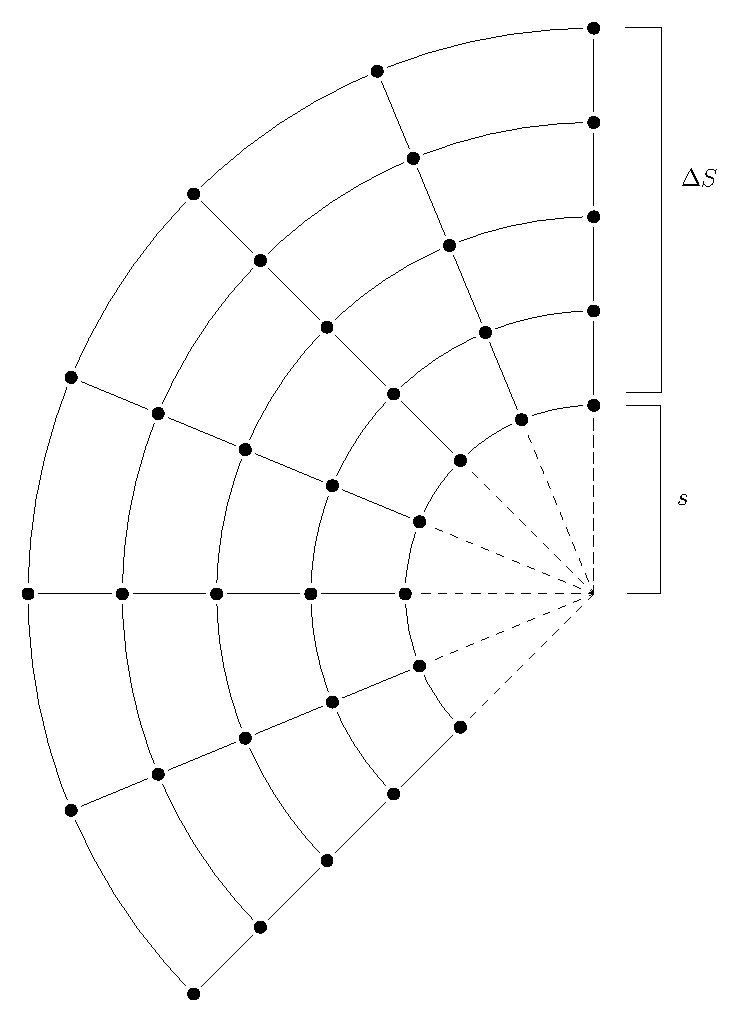
\includegraphics[scale=.6]{images/calibrationPattern2.eps}
	\caption{Kalibrierungsmuster mit $n = xxx, m = xxx$}
	\label{fig:calibrationPattern}
\end{figure}

warum gerade dieses muster? warum ist das so gut? wie berechnet man das muster? welche eigenschaften hat es?

Bilder von kegel mit muster drin?

wichtig das oben und unten etwas rand

\begin{figure}[!htb]
	\centering
	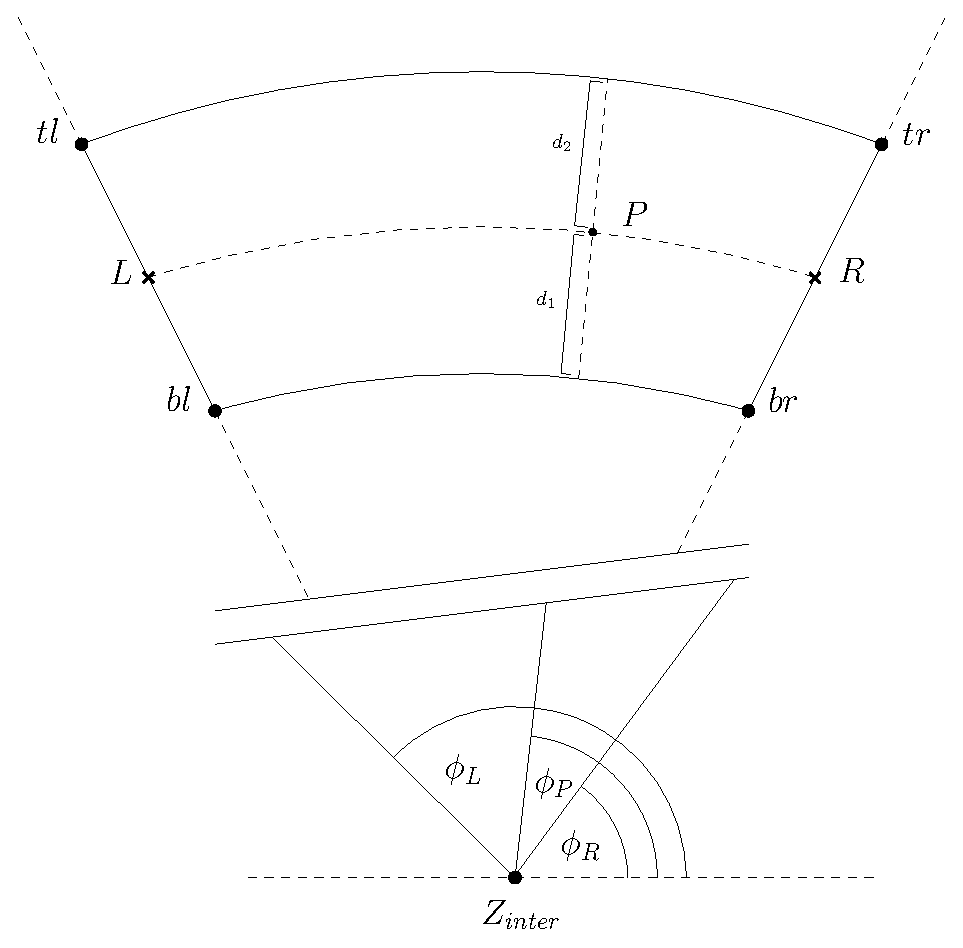
\includegraphics[scale=.6]{images/radialInterpolation.eps}
	\caption{Interpolation}
	\label{fig:Interpolation}
\end{figure}


warum ist das wichtig dass das ellipsenschätzen robust ist?
anzahl iterationen ransac
